前面在引入复数的时候,我们已经知道如何求解一元二次方程,其解为解析的.
经过数学家们的不断努力,三次方程及四次方程在16世纪中有了解答.
如一元三次方程 
$
a x^3+b x^2+c x+d=0, a \neq 0
$
的解也可解析求得.但是,一般五次及其以上的一元多项式方程无解析解,
称为Abel–Ruffini 定理.也就是说诸如
$x^5 - x -1 = 0$这样的方程也无法解析求出.
%伽罗华利用群论证明了一般,即.
此外,现实情况常常需要我们求解如$ e^x  =\cos x $这样的超越方程.因此,我们需要
依赖数值方法来求解这样的问题.这一部分,我们将主要探讨解决这类问题的方法.

\subsection{二分法 (Bisection method)}
我们以一个三次方程为例,看看我们有什么办法来求解.该方程为
$$
\frac{1}{1+x^2} = x 
$$
方程左右两边可以在图上画出(见图\ref{fig:cubic_equation}),图上可以大致预估
解的范围.
由代数基本定理,我们知道它必然有三个解,例如使用WolframAlpha可以得到实数解
为
$$
x=\frac{\sqrt[3]{2(9+\sqrt{93})}-2 \sqrt[3]{\frac{3}{9+\sqrt{93}}}}{6^{2 / 3}}
$$
数值解为
$$
 x \approx 0.6823278038280193273694837.
$$
\begin{figure}[ht]
    \centering
    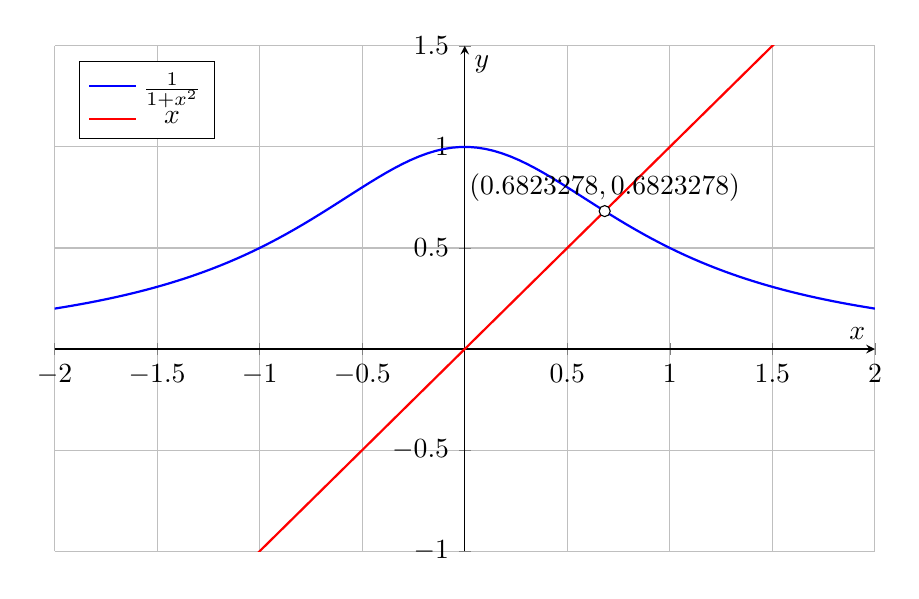
\begin{tikzpicture}
    \begin{axis}[
        axis lines = middle,
        grid = both,
        xlabel = {$x$},
        ylabel = {$y$},
        xmin = -2, xmax = 2,
        ymin = -1.0, ymax = 1.5,
        legend pos = north west,
        width = 12cm, height = 8cm,
        samples = 100,
        domain = -2:2,
    ]
    
    % Plot of 1/(1+x^2)
    \addplot[
        blue,
        thick,
    ]
    {1/(1 + x^2)};
    \addlegendentry{$\frac{1}{1 + x^2}$}

    % Plot of x
    \addplot[
        red,
        thick,
    ]
    {x};
    \addlegendentry{$x$}
    
    % Intersection point
    \addplot[
        mark=*,
        mark options={fill=white},
        only marks,
        nodes near coords,
        point meta=explicit symbolic
    ] coordinates {
        (0.6823278,0.6823278) [$(0.6823278, 0.6823278)$]
    };
    
    \end{axis}
\end{tikzpicture}
    \caption{三次方程$\frac{1}{1+x^2} = x$示意图.}
    \label{fig:cubic_equation}
\end{figure}

下面我们将使用\textbf{试错法}来看看是否可以给出比较满意的答案.
我们将试错的过程记录下来做成一个表格方便分析(见表\ref{tab:trial_error}).为此,
方程左侧记为left-hand side (L.H.S.),右侧记为
right hand side (R.H.S.).
当方程左右两端的差为正和负的情况,插值的方法很奏效,并且可以继续进行下去,直到得到满意的结果.
\renewcommand{\arraystretch}{1.5} % Increase row height for vertical centering
\begin{table}[ht]
    \centering
    \caption{试错法范例过程.}
    \label{tab:trial_error}
    \begin{tabular}{p{1cm}| >{\centering\arraybackslash}p{8cm}|>{\centering\arraybackslash}p{1cm}|p{1cm}p{1cm}p{1cm}}
        \hline
        步骤 & 思考 & $x$ & L.H.S. & R.H.S & 差 \\ \hline
        1.& 尝试$x=0$  & 0 & 1.0 & 0.0 &  1.0 \\ \hline
        2.& 不好,试一下$x=1$? & 1 & 0.5 &  1.0 & -0.5 \\ \hline
        3.& 也不是很妙! 但是差或正或负,也许结果在中间?
        不如试一下$x=0.5$
         & 0.5 & 0.8 & 0.5 &  0.3 \\ \hline
        4.& 差更接近了,不错,试一试$x=0.7$
         & 0.7 & 0.671 & 0.7 & −0.029 \\ \hline
        5.& 步骤3和4的结果也有正有负,试一试二者之间插值?
        $x = 0.7-0.2\frac{0.029}{0.3+0.029} \approx 0.6824$  
        & 0.6824 & 0.6823 & 0.6824 & -0.001 \\ \hline
    \end{tabular}
\end{table}
\renewcommand{\arraystretch}{1.0} % Increase row height for vertical centering

上述方法稍加修改便可以利用计算机进行处理了,这种方法成为\textbf{二分法}(bisection method),
是一种方程式根的近似值求法.其算法可以总结如下:
\\
若要求已知函数 $f(x)=0$ 的根 ( $x$ 的解), 则:
\begin{enumerate}
    \item  先找出一个区间 $[a, b]$, 使得 $f(a)$ 与 $f(b)$ 异号.根据介值定理,这个区间内一定包含着方程式的根.
    \item  求该区间的中点 $m=\frac{a+b}{2}$, 并找出 $f(m)$ 的值.
    \item  若 $f(m)$ 与 $f(a)$ 正负号相同则取 $[m, b]$ 为新的区间, 否则取 $[a, m]$.
    \item  重复第 2 和第 3 步至理想精确度为止.
\end{enumerate}
该方法很容易实现,但它有多好?是不是总是好用呢?如果好用,多快能收敛到正确的解?
为此,我们需要定义收敛的阶数和速率来回答这些问题.
在数值分析中,收敛性是一个重要的概念.
% 我们通常希望一个数值方法能以尽可能快的速度收敛到真实解.
% 本文将详细讨论收敛阶数和收敛速率这两个重要概念,
% 并给出相关例题和课后习题.

\begin{definition}
    设 $\{x_k\}$ 是一个收敛于$x^*$的数列.
    当$p>1$, 对于常数 $r\in (0, \infty)$, 
    或当$p=1$,对于常数 $r\in (0, 1)$, 
    有
\begin{equation}
    \lim_{k\to \infty} \frac{|x_{k+1} - x^*| } {|x_k - x^*|^p} = r
\end{equation}
% |x_{k+1} - x^*| \leq r |x_k - x^*|^p,
那么我们称 $\{x_k\}$ 以 $p$ 阶收敛到 $x^*$.
这里,$p$ 被称为\textbf{收敛阶数}, $r$被称为\textbf{收敛速率}.
\end{definition}
这里注意,$p$不一定为整数.例如割线法(secant method)以$p\approx 1.618$阶收敛.
\begin{itemize}
    \item 当 $p = 1$ 时,
        \begin{itemize}
            \item 如果 $r < 1$,我们称收敛是\textbf{线性(linear)}的;
            \item 如果 $r = 1$,我们称收敛是\textbf{亚线性(sublinear)}的;
            \item 如果 $r = 0$,我们称收敛是\textbf{超线性(superlinear)}的;
        \end{itemize}
    \item 当 $p = 2$ 时,我们称收敛是\textbf{二次(quadratic)}的;
    \item 当 $p = 3$ 时,我们称收敛是\textbf{三次(cubic)}的;
    \item 一般地,当 $p > 1$ 时,$p$ 越大,收敛越快.
\end{itemize}

在数值分析中,如果一个迭代方法产生的连续近似值在初始近似值已经足够接近解时保证收敛到解,
那么称该方法
\textbf{局部收敛}.对于非线性方程迭代求解方法,如牛顿法,通常仅是局部收敛的.
如果一个迭代方法对于任意初始近似值都能收敛,那么称该方法\textbf{全局收敛}.
对于线性方程组的迭代方法通常是全局收敛的.

\begin{table}[ht]
    \centering
    \caption{一些收敛数列的性质.}
    \label{tab:convergent_sequences}
\begin{tabular}{lccc}
    \hline 收敛性 & 数列 & 收敛速率 & $k \rightarrow \infty$ \\
    \hline sublinear & $1, \frac{1}{2}, \frac{1}{3}, \frac{1}{4} \ldots, k^{-1}, \ldots$ & $\frac{(k+1)^{-1}}{k^{-1}}$ & 1 \\
    linear & $1, \frac{1}{2}, \frac{1}{4}, \frac{1}{8} \ldots, 2^{-k}, \ldots$ & $\frac{2^{-(k+1)}}{2^{-k}}$ & $\frac{1}{2}$ \\
    superlinear & $1, \frac{1}{4}, \frac{1}{27}, \frac{1}{256} \ldots, k^{-k}, \ldots$ & $\frac{(k+1)^{-k-1}}{k^{-k}}$ & 0 \\
    quadratic & $1, \frac{1}{16}, \frac{1}{256}, \frac{1}{65536} \ldots, 2^{-k^2}, \ldots$ & $\frac{2^{-(k+1)^2}}{\left(2^{-k^2}\right)^{p=2}}$ & 1 \\
    \hline
\end{tabular}
\end{table}

让我们回到二分法,初始区间$I^{(0)} = [a,b]$, 其大小为$|I^{(0)}| = |b-a|$,
而随后的区间大小总是前一区间的一半.记第$k$步的误差为$e^{(k)} = x^{(k)} - x^*$,
那么
\begin{equation}
    |e^{(k)}| \leq |I^{(k)}| =  \half |I^{(k-1)}| = \frac{1}{4} 
    |I^{(k-2)}| \cdots = 2^{-k} | b-a|.
\end{equation}
容易看出该方法为线性收敛,且收敛速率为$\half$. 假设初始区间大小为$\epsilon_0$,
那么经过$k$步迭代后,误差$|e^{(k)}| \leq 2^{-k} \epsilon_0$.
那么我们大约需要多少步后能达到误差小于$\epsilon$?
不难分析得到,
我们需要
$$
 k = [ \log_2 (\epsilon_0/\epsilon)]
$$
次迭代.

虽然二分法收敛相对较慢,但好处是它是全局收敛的.通常可以将其与其他局域且快速收敛(如牛顿法)的方法
配合使用,以达到较为理想的结果.

\begin{example}
    求解方程 $f(x) = x^3 - x - 2 = 0$ 在区间 $[1, 2]$ 上的一个零点.
\begin{solution}
\begin{enumerate}
    \item[步骤1:] 初始区间 $[a, b] = [1, 2]$,计算 $f(a)$ 和 $f(b)$:
    \[
    f(1) = 1^3 - 1 - 2 = -2, \quad f(2) = 2^3 - 2 - 2 = 4.
    \]
    因为 $f(1)f(2) < 0$,满足二分法的应用条件.
    \item[步骤2:] 计算区间中点 $m$:
    \[
    m = \frac{1 + 2}{2} = 1.5.
    \]
    计算 $f(m)$:
    \[
    f(1.5) = 1.5^3 - 1.5 - 2 = -0.125.
    \]
    因为 $f(1)f(1.5) < 0$,新的区间为 $[1, 1.5]$.
    \item[步骤3:] 重复上述步骤,继续计算新的中点和函数值,直到找到足够精确的零点.

    \[
    \begin{aligned}
    m_1 &= \frac{1 + 1.5}{2} = 1.25, \quad f(1.25) = 1.25^3 - 1.25 - 2 = -1.296875, \quad \text{区间为} [1.25, 1.5], \\
    m_2 &= \frac{1.25 + 1.5}{2} = 1.375, \quad f(1.375) = 1.375^3 - 1.375 - 2 = -0.478516, \quad \text{区间为} [1.375, 1.5], \\
    m_3 &= \frac{1.375 + 1.5}{2} = 1.4375, \quad f(1.4375) = 1.4375^3 - 1.4375 - 2 = 0.053711, \quad \text{区间为} [1.375, 1.4375], \\
    m_4 &= \frac{1.375 + 1.4375}{2} = 1.40625, \quad f(1.40625) = 1.40625^3 - 1.40625 - 2 = -0.164795, \quad \text{区间为} [1.40625, 1.4375], \\
    m_5 &= \frac{1.40625 + 1.4375}{2} = 1.421875, \quad f(1.421875) = 1.421875^3 - 1.421875 - 2 = -0.056396, \quad \text{区间为} [1.421875, 1.4375].
    \end{aligned}
    \]
    继续迭代,最终可以找到一个足够精确的零点.
\end{enumerate}
\end{solution}

\end{example}

\subsection{牛顿法 (Newton's method)}
\label{sub:newton_method}

\begin{theorem}[Taylor Theorem]
    若函数$f:\mathbb{R} \to \mathbb{R}$二阶连续可微,
    有
    \begin{equation}
        f(x+p) = f(x) + f'(x) p + \half f''(x + t p) p^2
    \end{equation}
    其中$t\in (0,1)$.
\end{theorem}
若$x^*$是$f(x)$的零点,即取$x=x^*$, $p$足够小, 则有
$$
f(x^*+p) = f(x^*) + f'(x^*) p + \half f''(x^* + t p) p^2
$$



考虑方程 $f(x) = x^2 - 2 = 0$,其根为 $\sqrt{2}$.牛顿法的迭代公式为:
\[
x_{k+1} = x_k - \frac{f(x_k)}{f'(x_k)} = x_k - \frac{x_k^2 - 2}{2x_k} = \frac{x_k}{2} + \frac{1}{x_k}.
\]

假设初始值 $x_0 = 1.5$,我们可以计算前几次迭代:
\[
\begin{aligned}
x_1 &= \frac{1.5}{2} + \frac{1}{1.5} = 1.4167, \\
x_2 &= \frac{1.4167}{2} + \frac{1}{1.4167} = 1.4142, \\
x_3 &= \frac{1.4142}{2} + \frac{1}{1.4142} = 1.4142.
\end{aligned}
\]

我们看到,迭代值逐渐接近 $\sqrt{2} \approx 1.4142$.然而,如果初始值选择得不好,例如 $x_0 = 0.1$,可能会导致不收敛.因此,牛顿法是局部收敛的.

\section*{全局收敛}

如果一个迭代方法对于任意初始近似值都能收敛,那么称该方法为全局收敛.对于线性方程组的迭代方法通常是全局收敛的.

\paragraph{例子2:雅可比迭代法}
考虑线性方程组
\[
\begin{cases}
3x + y = 5, \\
x + 2y = 5.
\end{cases}
\]

用雅可比迭代法求解该方程组,其迭代公式为:
\[
\begin{aligned}
x_{k+1} &= \frac{5 - y_k}{3}, \\
y_{k+1} &= \frac{5 - x_k}{2}.
\end{aligned}
\]

假设初始值 $x_0 = 0, y_0 = 0$,我们可以计算前几次迭代:
\[
\begin{aligned}
x_1 &= \frac{5 - 0}{3} = 1.6667, \\
y_1 &= \frac{5 - 0}{2} = 2.5, \\
x_2 &= \frac{5 - 2.5}{3} = 0.8333, \\
y_2 &= \frac{5 - 1.6667}{2} = 1.6667.
\end{aligned}
\]

我们看到迭代值逐渐接近方程组的解 $x = 1, y = 2$.无论初始值如何选择,雅可比迭代法都会收敛到解.因此,雅可比迭代法是全局收敛的.





收敛速率是指数列 $\{x_k\}$ 收敛到极限 $x^*$ 的速度.一个常用的量化收敛速率的方法是定义收敛因子 $\rho$,使得

\[
|x_{k+1} - x^*| \approx \rho |x_k - x^*|,
\]
其中 $\rho$ 是一个常数.当 $\rho < 1$ 时,数列 $\{x_k\}$ 收敛.

具体地,如果 $\{x_k\}$ 以线性速度收敛,那么有
\[
|x_{k+1} - x^*| \leq \rho |x_k - x^*|,
\]
其中 $\rho \in (0, 1)$.

当收敛是二次的,即 $p = 2$,收敛速率通常表现为
\[
|x_{k+1} - x^*| \leq r |x_k - x^*|^2,
\]
这种情况下,误差平方级别地减小,收敛非常快.

\section*{例题}

\paragraph{例题1:}
设 $\{x_k\}$ 是一个数列,其满足
\[
|x_{k+1} - x^*| \leq 0.5 |x_k - x^*|,
\]
其中 $x^* = 2$.证明该数列线性收敛,并计算当 $x_0 = 3$ 时前五次迭代的误差.

\textbf{解:}
根据题意,收敛因子 $\rho = 0.5$,且初始误差为
\[
|x_0 - x^*| = |3 - 2| = 1.
\]
每次迭代的误差分别为:
\[
\begin{aligned}
|x_1 - x^*| &\leq 0.5 |x_0 - x^*| = 0.5 \times 1 = 0.5, \\
|x_2 - x^*| &\leq 0.5 |x_1 - x^*| = 0.5 \times 0.5 = 0.25, \\
|x_3 - x^*| &\leq 0.5 |x_2 - x^*| = 0.5 \times 0.25 = 0.125, \\
|x_4 - x^*| &\leq 0.5 |x_3 - x^*| = 0.5 \times 0.125 = 0.0625, \\
|x_5 - x^*| &\leq 0.5 |x_4 - x^*| = 0.5 \times 0.0625 = 0.03125.
\end{aligned}
\]
因此,该数列以线性速度收敛.

\paragraph{例题2:}
设 $\{x_k\}$ 是一个数列,其满足
\[
|x_{k+1} - x^*| \leq r |x_k - x^*|^2,
\]
其中 $r > 0$ 且 $x^* = 1$.证明该数列二次收敛,并计算当 $x_0 = 0.5$ 且 $r = 2$ 时前四次迭代的误差.

\textbf{解:}
根据题意,初始误差为
\[
|x_0 - x^*| = |0.5 - 1| = 0.5.
\]
每次迭代的误差分别为:
\[
\begin{aligned}
|x_1 - x^*| &\leq 2 |x_0 - x^*|^2 = 2 \times (0.5)^2 = 0.5, \\
|x_2 - x^*| &\leq 2 |x_1 - x^*|^2 = 2 \times (0.5)^2 = 0.5, \\
|x_3 - x^*| &\leq 2 |x_2 - x^*|^2 = 2 \times (0.5)^2 = 0.5, \\
|x_4 - x^*| &\leq 2 |x_3 - x^*|^2 = 2 \times (0.5)^2 = 0.5.
\end{aligned}
\]
因此,该数列以二次速度收敛.

\section*{课后习题}

\paragraph{习题1:}
设 $\{x_k\}$ 是一个数列,其满足
\[
|x_{k+1} - x^*| \leq 0.8 |x_k - x^*|,
\]
其中 $x^* = 0$.证明该数列线性收敛,并计算当 $x_0 = 1$ 时前五次迭代的误差.

\paragraph{习题2:}
设 $\{x_k\}$ 是一个数列,其满足
\[
|x_{k+1} - x^*| \leq r |x_k - x^*|^3,
\]
其中 $r > 0$ 且 $x^* = 2$.证明该数列三次收敛,并计算当 $x_0 = 1$ 且 $r = 1$ 时前三次迭代的误差.

\paragraph{习题3:}
设 $\{x_k\}$ 是一个数列,其满足
\[
|x_{k+1} - x^*| \leq 0.9 |x_k - x^*|,
\]
其中 $x^* = 3$.证明该数列线性收敛,并计算当 $x_0 = 4$ 时前四次迭代的误差.

\section*{总结}

理解收敛阶数和收敛速率有助于评估数值方法的效率.
高阶收敛方法通常比低阶收敛方法更有效,因为它们能够在更少的迭代次数内达到相同的精度.然而,高阶方法可能更复杂,计算成本也更高.
因此,在实际应用中,需要在收敛速度和计算成本之间做出权衡.





